\documentclass[a4paper,12pt,openany,oneside,header=optiontohead]{scrbook} % kodovanie diakritiky je utf-8
\usepackage[utf8]{inputenc}
\usepackage[slovak]{babel}
\usepackage{a4wide,color}
\usepackage[includehead, includefoot,top=2.5cm, bottom=2.5cm, left=2.75cm, right=2.75cm]{geometry}
%\usepackage[includehead, includefoot, top=2.5cm, bottom=2.5cm, left=3.5cm, right=2cm]{geometry}
\usepackage{lmodern}
\usepackage[T1]{fontenc}
\usepackage{fontenc}
\usepackage{amsfonts}
\usepackage{amssymb}
\usepackage{epsfig}
\usepackage{wrapfig}
\usepackage{graphicx}
\usepackage{caption}
\usepackage{subcaption}
\usepackage{url}
\usepackage[bookmarks]{hyperref}
\usepackage{amsmath}
\usepackage{amsthm}
\usepackage{dsfont}
\usepackage{mathrsfs}
\usepackage{bm} %pisat boldom v math-mode
\usepackage{fancyhdr}
\usepackage{indentfirst}
\usepackage{float}
\usepackage{enumitem}
\setlist{parsep=0pt,listparindent=\parindent} % aby sa v enumerate robili dobre odseky

\usepackage{pdfpages}
\usepackage{listings}
\renewcommand\baselinestretch{1.3} % riadkovanie jeden a pol

\definecolor{dkgreen}{rgb}{0,0.6,0}
\definecolor{gray}{rgb}{0.5,0.5,0.5}
\definecolor{mauve}{rgb}{0.58,0,0.82}

%definície pre foju
\newtheorem{veta}{Veta}[section] 
\newtheorem{df}[veta]{Definícia}
\newtheorem{lema}[veta]{Lema}
\newtheorem{dosledok}[veta]{Dôsledok}
\def\R{{\cal R}} % znak pre regulárne jazyky
\def\L{\mathscr{L}} % zvyšné triedy jazykov
\def\P{{\cal P}} % potenčná množina
\def\N{\mathds{N}} %prirodzene cisla
\def\le{LEregex}
\def\nle{nLEregex}
\def\e{Eregex}

% pekne pokope definujeme potrebne udaje
\def\mftitle{......názov.......}
\def\mftitlefirst{.........názov..........}
\def\mftitlesecond{}
\def\mfthesistype{Diplomová práca}
\def\mfauthor{Tatiana Tóthová}
\def\mfadvisor{RNDr. Michal Forišek, PhD.}
\def\mfdate{201.}
\def\mfplacedate{Bratislava, \mfdate}
\def\mfuniversity{Univerzita Komenského, Bratislava}
\def\mffakulta{Fakulta Matematiky, Fyziky a Informatiky}
% \ifx\pdfoutput\undefined\relax\else\pdfinfo{ /Title (\mftitle) /Author (\mfauthor) /Creator (PDFLaTeX) } \fi

\def\todo{{\color{red} TODO!!!}}
\def\method#1{{\tt #1}}

\ifpdf
  \pdfinfo{
    /Title (\mftitle)
    /Author (\mfauthor)
    /Creator (PDFLaTeX)
  }
\else
\fi

\begin{document}

\frontmatter

\thispagestyle{empty}

\noindent
%\begin{minipage}{0.20\textwidth}
%
\includegraphics[width=0.9\textwidth]{komlogo-new}
%\end{minipage}
\begin{center}
\begin{minipage}{0.8\textwidth}
\centerline{\renewcommand\baselinestretch{1.3} \LARGE\sc\mfuniversity}
\centerline{\sc\mffakulta}
\end{minipage}
\end{center}

\vfill
\begin{center}
\begin{minipage}{1\textwidth}
%\hrule
\bigskip\bigskip
\begin{center}
\linespread{1}\LARGE\sc\mftitle
\end{center}
\smallskip
\centerline{\mfthesistype}
\bigskip
\bigskip
%\centerline{\large\sc\mfauthor}
\bigskip\bigskip
%\hrule
\end{minipage}
\end{center}
\vfill
{\bf
\begin{minipage}{0.4\textwidth}
\begin{flushleft} \large
~\mfdate
\end{flushleft}
\end{minipage}
\begin{minipage}{0.59\textwidth}
\begin{flushright} \large
\indent\mfauthor
\end{flushright}
\end{minipage}
}
%{\bf Vedúci:} \mfadvisor
\eject % EOP i

% \thispagestyle{empty}~\vfill\eject % EOP ii % zadna strana obalu je prazdna

\thispagestyle{empty}

\noindent
%\begin{minipage}{0.20\textwidth}
%
\includegraphics[width=0.9\textwidth]{komlogo-new}
%\end{minipage}
\begin{center}
\begin{minipage}{0.8\textwidth}
\centerline{\LARGE\sc\mfuniversity}
\centerline{\sc\mffakulta}
\end{minipage}
\end{center}

\vfill
\begin{center}
\begin{minipage}{1\textwidth}
%\hrule
\bigskip\bigskip
\begin{center}
\linespread{1}\LARGE\sc\mftitle
\end{center}
\smallskip
\centerline{\mfthesistype}
\bigskip
\bigskip
%\centerline{\large\sc\mfauthor}
\bigskip\bigskip
%\hrule
\end{minipage}
\end{center}
\vfill
\begin{minipage}{0.8\textwidth}
\begin{tabular}{l l}
Študijný program:& Informatika \\
Študijný odbor:& .... Informatika \\
Školiace pracovisko:& Katedra Informatiky\\
Školiteľ:&   \mfadvisor \\
\end{tabular}
\end{minipage}
\begin{center}
\end{center}
\vfill
{\bf
\begin{minipage}{0.4\textwidth}
\begin{flushleft} \large
~\mfplacedate
\end{flushleft}
\end{minipage}
\begin{minipage}{0.59\textwidth}
\begin{flushright} \large
\indent\mfauthor
\end{flushright}
\end{minipage}
}
%{\bf Vedúci:} \mfadvisor
\eject % EOP iii

% \thispagestyle{empty}~\vfill\eject % EOP iv % zadna strana titulky je prazdna

% {~}\vspace{12cm}
% 
% \noindent
% \begin{minipage}{0.25\textwidth}~\end{minipage}
% \begin{minipage}{0.68\textwidth}
% Čestne prehlasujem, že som túto diplomovú prácu vypracoval(a) samostatne s použitím citovaných zdrojov.
% 
% \bigskip\bigskip
% 
% \hfill\hbox to 6cm{\dotfill}
% \end{minipage}
% \vfill\eject % EOP v
% ~\vfill\eject % EOP vi % zadna strana prehlasenia je prazdna

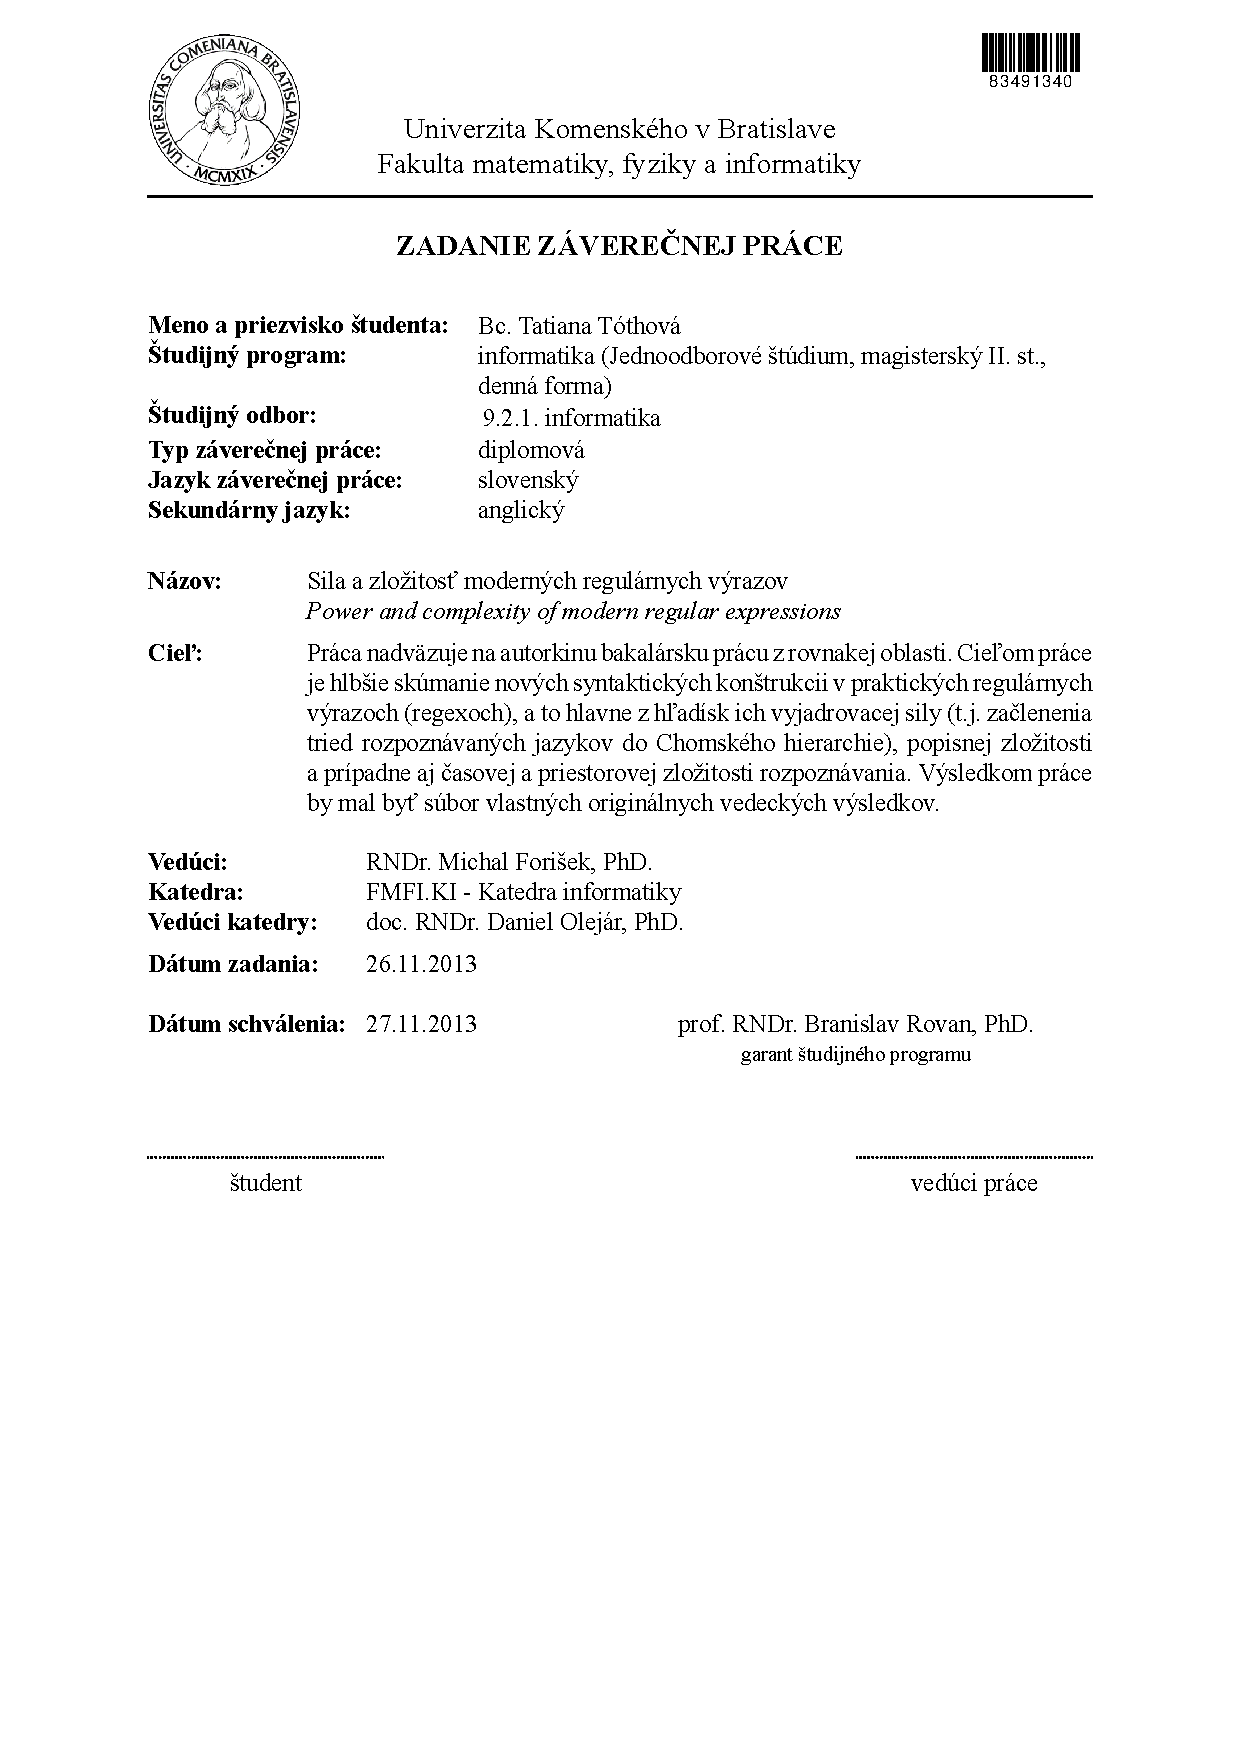
\includepdf{zadanie.pdf}

\pagestyle{plain}

{~}\vspace{12cm}

\noindent
\begin{minipage}{0.25\textwidth}~\end{minipage}
\begin{center}
\begin{minipage}{1\textwidth}
\textit{.....tu bude poďakovanie.....}
\end{minipage}
\end{center}
\hfill\textit{\mfauthor}
\vfill\eject % EOP v
% ~\vfill\eject % EOP vi % zadna strana prehlasenia je prazdna


\noindent
%\begin{minipage}{0.25\textwidth}~\end{minipage}
\begin{center}
\begin{minipage}{1\textwidth}
\centerline{\large Abstrakt}
%\begin{center}
\input abstraktSK.tex
\\ \\ 
{\bf Kľúčové slová:} nejaké, kľúčové, slová
%\end{center}
\end{minipage}
\end{center}
\eject % EOP v
% ~\vfill\eject % EOP vi % zadna strana prehlasenia je prazdna

\noindent
%\begin{minipage}{0.25\textwidth}~\end{minipage}
\begin{center}
\begin{minipage}{1\textwidth}
\centerline{\large Abstract} 
%\begin{center}
\input abstraktEN.tex
\\ \\
{\bf Key words:} some, key, words
%\end{center}
\end{minipage}
\end{center}
\eject % EOP v
% ~\vfill\eject % EOP vi % zadna strana prehlasenia je prazdna

\tableofcontents

\mainmatter
\pagestyle{fancy}

\input uvod.tex
\input kapitola1.tex
\input vysledky.tex
\input zaver.tex

\backmatter

%\cleardoublepage
\phantomsection
\addcontentsline{toc}{chapter}{Literatúra}
\nocite{*}
\bibliographystyle{alpha}
\bibliography{literatura.bib}

\end{document}
